\chap{Evaluation of a Novel Behaviour Change App through Expert Review} \label{chapter: prevention-evaluation}

\epigraph{The most important property of a program is whether it accomplishes the intention of its user.}{\textit{Charles Antony Richard Hoare}}

This Chapter details the results of a series of assessments of the developed Gray Matters app. Ranging from expert review to content analysis, the app and its components are critically evaluated. These evaluations result in the exposure of common attributes amongst successful apps, which influence future recommendations of various software elements and approaches.

\section{Introduction}
Following the process outlined in Section \ref{subsection: framework-process}, the developed solution should be peer-reviewed by domain experts using a suitable objective method. Academically recognised approaches for the assessment of mHealth apps are very limited, however, the previously introduced MARS \cite{Stoyanov2015} tool is a suitable scale by which the Gray Matters app can be evaluated.

\section{Mobile App Rating Scale}
The MARS tool provides an established set of methods by which to rate an app across 4 objective criteria: Engagement, Functionality, Aesthetics, and Information. The scale also includes an additional subjective quality assessment criteria. Twenty-three individual criterion are presented to the reviewer in total, each relating to a specific criteria, and a mean score is generated for each. A summary score, referred to as the MARS mean score, is calculated as the mean score across the 4 objective criteria (excluding the subjective quality criteria scores). This is the primary measure by which all apps are contrasted or ranked.
In the development of the MARS framework, the authors identified 59 mHealth (mobile health) apps that were available to the public via their platform's respective app stores. Of these 59, 9 were randomly selected to develop the scale in a pilot study, and 50 were subsequently used to evaluate the consistency and inter-reliability of the scale.

\subsubsection{Potential Limitations}
Whilst the MARS framework provides a suitable set of objective questions, and displayed excellent internal consistency, a number of limitations with the framework were observed.

\textbf{Stress Domain Focused.}
The original rating scale was developed during a pilot study, by reviewing 9 apps, of which only 1 addressed more than one behavioural domain. A large proportion of these apps, 66.7\%, were primarily aimed at reducing stress, whilst the remainder addressed diet, sleep and social domains. No apps addressed physical activity, diet, or smoking.

\textbf{Excludes N/A Ratings.}
Within the information criteria rating scale, questions aim to score various aspects of the information provided, e.g., quality, quantity, graphical representation etc. This is performed by rating these sub-categories from 1-5. The highest rating of 5 denotes that the information is correct, clear and concise. The lowest rating of 1, however, is reserved for irrelevant or incorrect information. There is no figure that denotes a lack of information, or no information. The framework states that if this occurs, that they should be marked `N/A' for not applicable, and these should be excluded when calculating the mean information score. This is problematic for a number of reasons.
Many mHealth and educational apps attempt to deliver information in a number of formats, using text, audio, video and graphs. However, if a low quality app were to provide no information, yet match their marketplace description, it is still possible for the app to score a high mean information score due to the exclusion of N/A entries. An illustrative example of this is presented in Table \ref{tbl: information-rating-illustration}.

\begin{table}[]
\centering
\caption{Example of N/A label bias on mean information score.}
\label{tbl: information-rating-illustration}
\resizebox{\textwidth}{!}{%
\begin{tabular}{@{}cclllllll@{}}
\toprule
 & \multicolumn{1}{m{2.3cm}}{\centering App Description Accuracy} & Goals & Quality & Quantity & Visual & Credibility & Evidence & \multicolumn{1}{m{1.2cm}}{\centering Mean Score} \\ \midrule
App A       & 3                        & 3     & 4       & 3        & 3      & 1           & N/A      & {\it 2.83} \\
App B       & 5                        & N/A   & N/A     & N/A      & N/A    & 1           & N/A      & {\it 3.00} \\ \bottomrule
\end{tabular}
}
\end{table}

\textbf{Disciplinary Bias.}
In the pilot study, the apps were reviewed by 2 expert raters from the field of psychology. Upon examining the distribution of scoring from the pilot study, as presented in Figure \ref{fig: mars-pilot-histogram}, indicates that most apps scored above the scales natural mean point of 2.5. \begin{figure}[t]
    \centering
    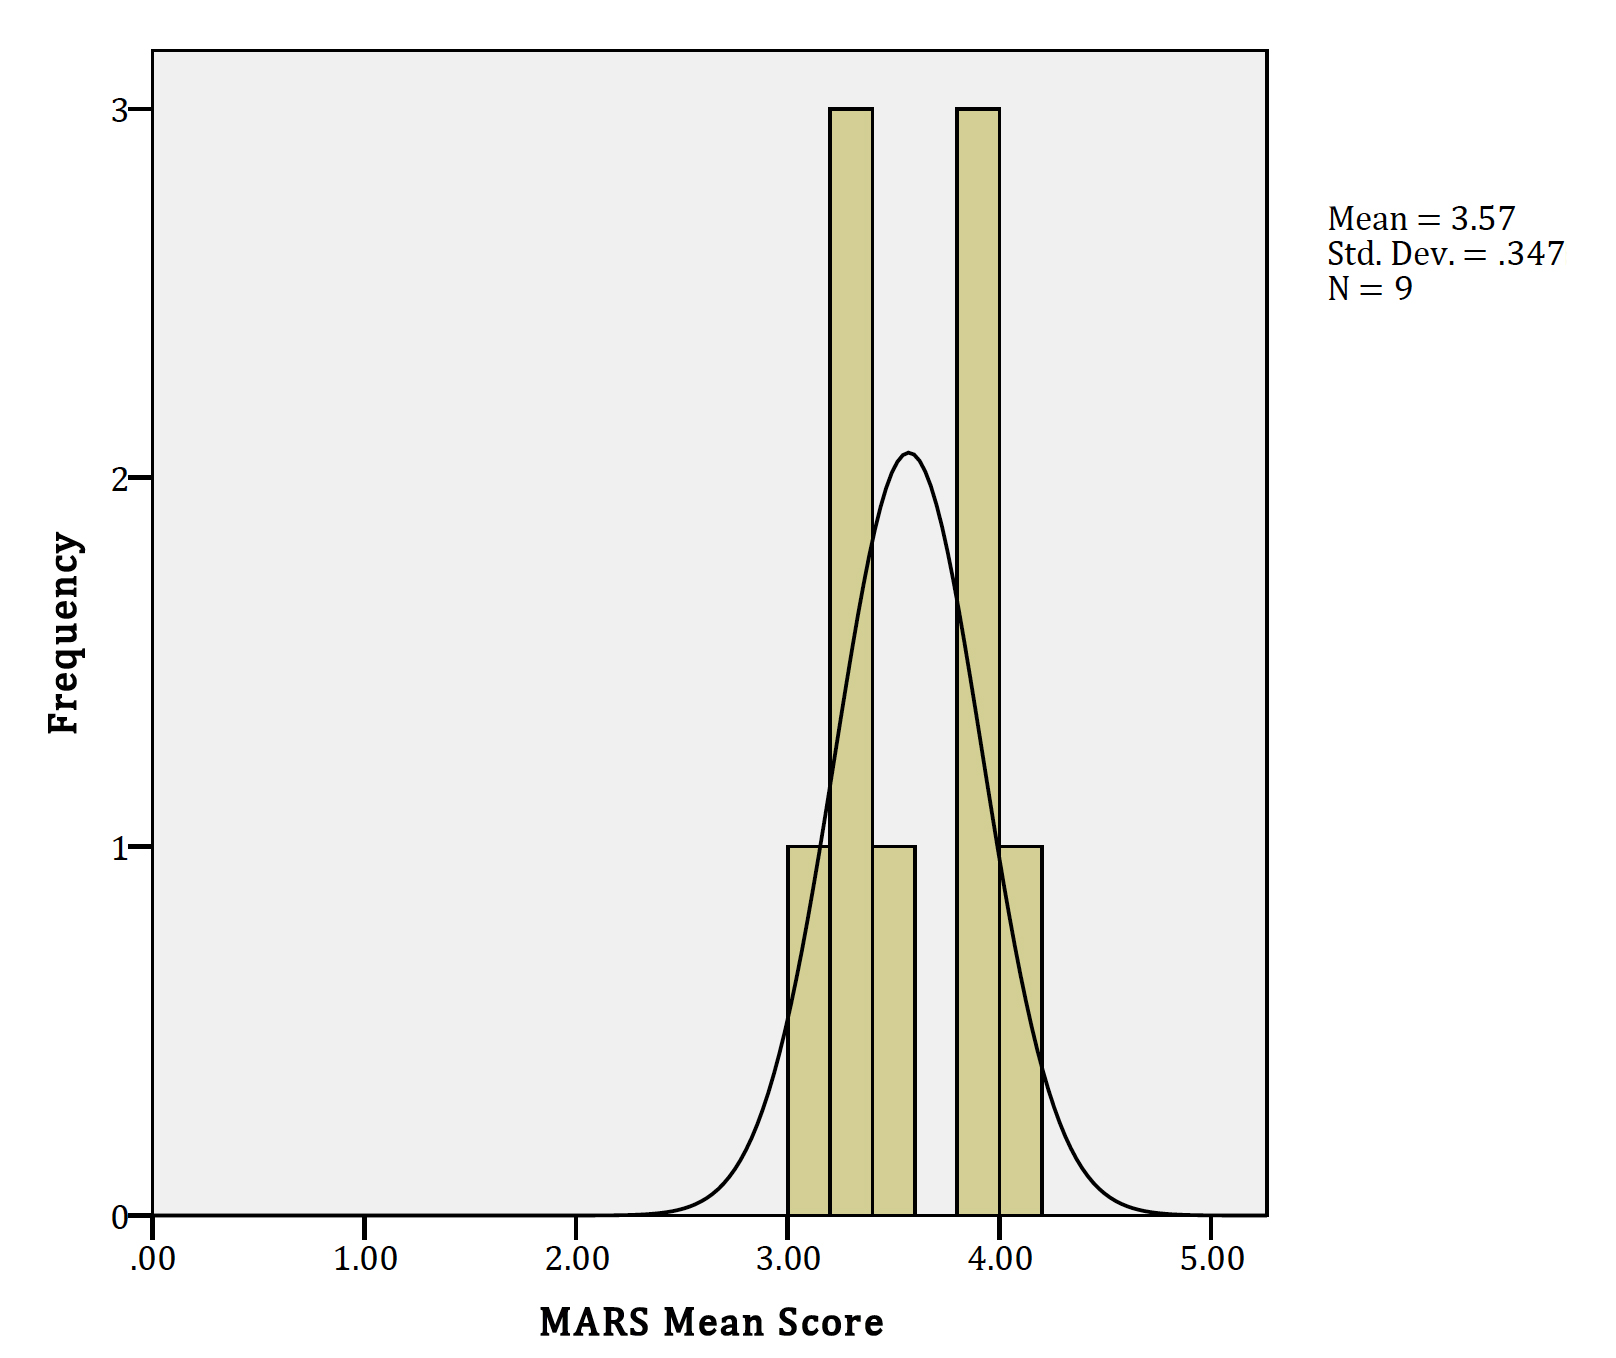
\includegraphics[scale=0.20, angle=0]{Files/prevention-study-2/figures/mars-pilot-histogram}
    \caption{Histogram showing distribution and normal curve of mean scores in initial MARS Pilot study.}
    \label{fig: mars-pilot-histogram}
\end{figure}
This hinted that cognitive bias may exist in the results, perhaps stemming from non-technologists scoring technology solutions highly due to lack of domain knowledge. The authors do state however that one reviewer has 9 years experience with information technology \cite{Stoyanov2015}, although the exact details of their proficiency was not stated.

\subsubsection{Testing for Disciplinary Bias}
To ensure this cognitive bias did not exist, the same 9 apps used to develop the MARS scale were evaluated by the author of this Thesis. Following the protocol of the original study \cite{Stoyanov2015}, all 9 apps were downloaded onto their respective platforms, used for approximately 10 minutes, and scored. The full assessment results sheet have been included in Appendix \ref{apndx: mars-pilot-reevaluation}.

The authors of the original study disclosed the criteria scores for each app, allowing for a detailed comparison. The resulting MARS scores from the pilot and the re-evaluation performed by the author can be found in Table \ref{tbl: MARSpilot-vs-author}.

\begin{table}[h]
\centering
\caption{MARS scores of initial 9 apps from Pilot study, as marked by original study and author.}
\label{tbl: MARSpilot-vs-author}
\resizebox{\textwidth}{!}{%
\begin{tabular}{@{}llll@{}}
\toprule
App & Score (MARS Pilot) & Score (Author) & Difference \\ \midrule
Breathe Daily & 3.91         & 3.75          & .16        \\
Everyday	Health with Acupressure & 3.52         & 3.63          & -.11       \\
Interpersonal Dynamics & 3.94         & 3.90          & .04        \\
iPhoria Nature's Music & 3.74         & 3.53          & .21        \\
iThoughtjournal & 3.65         & 3.51          & .14        \\
Meditation Seconds Lite & 3.71         & 3.48          & .23        \\
Personal	 Remedies & 3.77         & 3.59          & .18        \\
Sleep Easily              & 3.90         & 3.81          & .09        \\
We Breathe & 3.90         & 3.75          & .15        \\ \bottomrule
\end{tabular}
}
\end{table}

A number of tests were performed to measure the reliability of the author's scoring, following methods outlined in \cite{McHugh2012}. Intraclass correlation coefficient (ICC) using Cronbach's alpha was performed on the scores from both assessments, resulting in a correlation coefficient of .852, as presented in Table \ref{tbl: intraclass-pilot-reevaluation}. A consistency of 85.2\% between the original study and the re-evaluation performed by the author is high, and notably higher than the ICC of .79 from the original MARS study \cite{Stoyanov2015}. This finding supports the original study's claim that the scale has excellent consistency and inter-rater reliability \cite{Stoyanov2015}. It is therefore presumed that the remaining 50 apps would be marked similarly, despite variation in the expert rater's discipline. This assumption is tested again, later within this Chapter.

\begin{table}[h]
\centering
\caption{Intraclass Correlation Coefficient for Pilot vs Re-evaluation.}
\label{tbl: intraclass-pilot-reevaluation}
\resizebox{\textwidth}{!}{%
\begin{tabular}{@{}llllllll@{}}
\toprule
\multicolumn{1}{c}{} & \multicolumn{1}{c}{\multirow{2}{*}{\begin{tabular}[c]{@{}c@{}}Intraclass \\ Correlation \textsuperscript{\textit{b}}\end{tabular}}} & \multicolumn{2}{c}{95\% CI} & \multicolumn{4}{c}{F Test with True Value 0} \\ \cmidrule(l){3-8}
 & \multicolumn{1}{c}{} & Lower & Upper & Value & df1 & df2 & Sig \\ \midrule
Single Measures & .742 \textsuperscript{\textit{a}} & .206 & .935 & 6.740 & 8 & 8 & .007 \\
Average Measures & .852 \textsuperscript{\textit{c}} & .342 & .967 & 6.740 & 8 & 8 & .007 \\ \bottomrule
\end{tabular}
}
\end{table}

\section{Recruitment}
The Gray Matters app was publicly demonstrated during the Technology and Dementia symposium at the 2015 Alzheimer's Association International Conference in Washington, D.C \cite{AlzheimersAssociation2015}. During this event, a number of physicians, pharmacologists, psychologists and technologists were interested in the app's potential use cases. Interested parties were given access to an online version of the MARS tool from which they could complete the survey. In addition, a number of technology researchers from the Smart Environments Research Group at the University of Ulster were also permitted to complete the survey.

\section{Assessment Scores}
As of January 2016, 5 expert raters have reviewed the app using the MARS tool. These raters are from 2 relevant disciplines, Medicine (n=4) and Computer Science (n=1). It must be noted that the expert raters in both fields have had professional experience in psychology and/or the study of behaviour change.
Each rater was asked to download the app and use for 5-10 minutes. After use of the app, the rater was asked to complete the MARS survey. The rater could reuse the app during the completion of the survey to minimise information recall error. The descriptive statistics of the Gray Matters app ratings are presented in Table \ref{tbl: gm-expert-ratings}

%VIVA: Chris comment - 5 expert raters?
% Is this low?  Be prepared to defned this number of reviewers and the limitations a small number may have on your findings
% Phillp - The MARS scale was built upon the ratings of 2 users, however, the questions were developed in such a way that agreement.

\begin{table}[h]
\centering
\caption{Descriptive statistics of expert raters scoring for each assessment category, and total means, including and excluding subjectivity.}
\label{tbl: gm-expert-ratings}
\begin{tabular}{@{}llllll@{}}
\toprule
Criteria      & N & Minimum & Maximum & Mean   & Std. Deviation \\ \midrule
Engagement    & 5 & 3.80    & 4.40    & 4.1200 & .30332         \\
Functionality & 5 & 4.25    & 4.75    & 4.5000 & .17678         \\
Aesthetics    & 5 & 4.67    & 5.00    & 4.7360 & .14758         \\
Information   & 5 & 4.29    & 4.71    & 4.4860 & .18783         \\
Subjective    & 5 & 3.25    & 4.00    & 3.6000 & .37914         \\
MARS Score    & 5 & 4.31    & 4.60    & 4.4580 & .14307         \\
True Mean     & 5 & 4.10    & 4.47    & 4.2880 & .17513         \\ \bottomrule
\end{tabular}
\end{table}

\textbf{MARS Score.}
The app received a mean overall MARS score of 4.45 $\pm$ .14.

\textbf{Engagement.}
The app received a mean engagement score of 4.12 $\pm$ .30.

\textbf{Functionality.}
The app received a mean functionality score of 4.5 $\pm$ .176.

\textbf{Aesthetics.}
The app received a mean aesthetics score of 4.73 $\pm$ .147.

\textbf{Information.}
The app received a mean information score of 4.48 $\pm$ .187.

\textbf{Subjective.}
The app received a mean score of 3.6 $\pm$ .379.
As to be expected the subjectivity score shows the greatest degree of standard deviation, hence its naming.

\textbf{True Mean (Including Subjective).}
The app received a true mean score of 4.28 $\pm$ .121. This score is lower than the official MARS score which does not account for the subjective criteria. The difference between the MARS score (M = 4.45, SD = 0.30) and True Mean (M = 4.28, SD = .121) score was found to be statistically significant in a paired samples t-Test at the p \textless 0.05 level [t(4) = 6.292, p = 0.03].

\subsection{Discussion}
The app scored very highly in all areas. A mean MARS score of 4.45 ranks the Gray Matters app 2\textsuperscript{nd} out of 60 reviewed apps (59 Original + Gray Matters app). When comparing the true mean scores (including subjective score), the app also ranks 2\textsuperscript{nd}. The nearest ranking app in both cases is `headspace', a structured meditation guide which was launched in 2010 \cite{HEADSPACE}. Headspace is marketed as \textit{`a gym membership for the mind}', and aims to reduce stress and increase mindfulness for it's users. The app has over 5 million installs on android devices alone. If the MARS score is indicative of public adoption, the resulting Gray Matters app demonstrates the framework's promise as an mHealth development platform.

\textbf{Ensuring validity.}
Whilst the results of the expert review are encouraging, steps must be taken to ensure that these ratings were valid and comparable to the original study. To do this, each expert was asked to rate an app from the original MARS study, and from a list of newly sourced apps. In the following Sections, the inter-rater reliability and ICC scores for each expert are established. 

\section{Comparison with Existing Apps}
Whilst the MARS scale has produced an average rating of 4.45 across 5 expert reviewers, the score exists without true context. It is important to compare this result with that of existing apps, which are aiming for similar outcomes. As such, a number of apps within the area of quantified-self and health improvement were considered for review.
%VIVA: Chris comment - Is this a biased selection of apps for the reviewers to engage with?  Should they not have made the selection themselves?
 

\subsection{Existing App Review Data}
As noted earlier, the apps reviewed in the MARS pilot (n=9) were predominately focused on the stress domain. In the full MARS study, an additional 50 apps were included in the assessment of the scale. The original authors disclosed the criteria scores and mean MARS score for each of these 50 apps. These apps were then targeted for inclusion in a comparison with the Gray Matters app. Initial content analysis of the apps found that a 13.5\% (n=8) were not relevant to behaviour change in any of the identified domains, or they did not aim to improve health outcomes. As such these 8 were excluded from further study. Of the remaining apps (n=51), the behavioural focus was heavily unbalanced, with 74.5\% (n=38) of the apps focusing strictly on the stress domain. In addition, no apps reviewed in the original MARS studies addressed smoking, and only 1 targeted the social domain. As such it was apparent that additional apps should be reviewed to provide a fairer and representative comparison of existing apps in the marketplace.

\subsection{Identifying Suitable Apps}
Identifying suitable apps to compare to the developed solution is difficult. The Gray Matters app is a disease specific app, utilising education delivery and behaviour tracking across numerous behavioural domains. The Gray Matters app is itself a relatively novel concept, thus narrowing the number of potential apps from which to compare. There are however a large number of apps that focus on specific behavioural areas, such as cognitive stimulation, diet monitoring, activity tracking, activity promotion and stress relief. There are also a number of apps that aim to disseminate information on AD and other areas of cognitive decline.
%VIVA: Chris comment -Do you not loose the baseline though if you go outside of the original 59 apps?  I am a bit confused about this given the start of the Chapter really stresses the benefits of having these scores!

Suitable apps for comparison were identified by searching the iOS and Android marketplaces for apps that that met the following criteria:
\begin{itemize}[noitemsep,topsep=0pt]
\item Encouraged behaviour change
\item Aimed to improve health status
\item Gamified behaviour change
\item Delivered condition specific health education
\end{itemize}

%VIVA: Chris -  Where did these criteria arise from and what search criteria did you use when searching the app stores?
This search unveiled over 70 publicly available apps, of which 36 where identified as suitable for comparison. The distribution of primary behavioural domains targeted by these additional apps are presented in Table \ref{tbl: app-dataset-frequencies}. The inclusion of these apps does help to balance the distribution of domains targeted from the original study, however, stress remains the most frequently targeted domain (47.1\%).

\begin{table}[h]
\centering
\caption{Comparison of app datasets and distribution of primary behavioural domain targeted.}
\label{tbl: app-dataset-frequencies}
\begin{tabular}{@{}lllllll@{}}
\toprule
\multirow{2}{*}{Domain} & \multicolumn{2}{l}{MARS} & \multicolumn{2}{l}{App Market} & \multicolumn{2}{l}{Consolidated} \\ \cmidrule(l){2-7}
                        & n        & \%            & n           & \%               & n          & \%              \\ \midrule
Physical                & 4        & 7.8         & 8           & 22.2           & 12         & 13.8          \\
Diet                    & 2        & 3.9         & 7           & 19.4           & 9          & 10.3          \\
Cognitive               & 2        & 3.9         & 7           & 19.4           & 9          & 10.3          \\
Sleep                   & 4        & 7.8         & 3           & 8.3            & 7          & 8.0           \\
Social                  & 1        & 2.0         & 4           & 11.1           & 5          & 5.7           \\
Stress                  & 38       & 74.5        & 3           & 8.3            & 41         & 47.1          \\
Smoking                 & 0        & 0.0         & 4           & 11.1           & 4          & 4.6           \\ \midrule
Total                   & 51       & 100.0       & 36          & 100.0          & 87         & 100.0         \\ \bottomrule
\end{tabular}
\end{table}

\subsection{Ensuring Reliability}
All 36 apps were reviewed by the author of this Thesis. As established earlier, the authors ICC was .852, showing excellent consistency with the original study. To further validate the scores that were attributed by the author, each expert rater, in addition to rating the Gray Matters app, were asked to rate an additional 3 apps:
\begin{enumerate}[noitemsep,topsep=0pt]
\item Two from the original MARS list \cite{Stoyanov2015}.
\item One from the additional 36 apps identified by the author of this Thesis.
\end{enumerate} 

A measure of inter-rater reliability, or concordance, was calculated between the original study reviewers and the expert reviewers, including the Thesis author. These measures seek to justify the ratings reached by the experts in their review of the Gray Matters app.
%VIVA: Chris - This is all a bit confusing!  Can you perhaps draw a flowchart of what happened?

\subsubsection{Method}
Each expert rater was asked to review two apps from the original study \cite{Stoyanov2015} and one from the additional 36 apps added by the author. A random number generator was used to select the app ids. The 3 apps highlighted for review were: PTSD Coach (MARS), Conscious (MARS), Water Your Body (Extra). The scores reached by each expert rater, including the original MARS scores and authors re-evaluation, can be found in Table \ref{tbl: expert-vs-author-apps}.

\begin{table}[h]
\centering
\caption{MARS scores attributed by each expert rater, the original study, and the author.}
\label{tbl: expert-vs-author-apps}
\resizebox{\textwidth}{!}{%
\begin{tabular}{@{}llllllll@{}}
\toprule
                & MARS & Expert 1 & Expert 2 & Expert 3 & Expert 4 & Expert 5 & Author \\ \midrule
PTSD Coach      & 4.29 & 3.1      & 3.26     & 3.63     & 3.1      & 3.12     & 3.1    \\
Conscious        & 3.36 & 2.93     & 3.38     & 3.26     & 3.15     & 3.3      & 3.15   \\
Water Your Body & N/A   & 3.7      & 3.77     & 4.11     & 3.96     & 3.85     & 3.96   \\
Gray Matters    & N/A   & 4.31     & 4.48     & 4.59     & 4.31     & 4.6      & N/A     \\ \bottomrule
\end{tabular}
}
\end{table}

\subsubsection{Expert Review and Original MARS Reliability}
Using the MARS scores from the original study and the scores from the expert reviews, a reliability analysis was performed. Descriptive statistics, detailing means and standard deviations for each rater are displayed in Table \ref{tbl: expert-vs-mars-apps-descriptive}. 

\begin{table}[h]
\centering
\caption{Expert rater and MARS statistics.}
\label{tbl: expert-vs-mars-apps-descriptive}
\begin{tabular}{@{}llll@{}}
\toprule
          & Mean   & Std. Deviation & N \\ \midrule
Expert 1  & 3.0150 & .12021         & 2 \\
Expert 2 & 3.3200 & .08485         & 2 \\
Expert 3 & 3.4450 & .26163         & 2 \\
Expert 4 & 3.1250 & .03536         & 2 \\
Expert 5 & 3.2100 & .12728         & 2 \\
MARS      & 3.8250 & .65761         & 2 \\ \bottomrule
\end{tabular}
\end{table}

In this instance, it can be noted that Expert 1 attributes the lowest mean scores across the reviewed apps (n=2), whilst the original MARS score has the highest mean and largest standard deviation. The differences between the MARS score and the experts seems significant. Reliability analysis performed using SPSS v22 confirms this, showing an ICC of .167. This suggests poor consistency between the experts and the original MARS study. It appears that the MARS study's results may be the cause of this. To test, reliability analysis was performed between the expert ratings of all apps (n=4), omitting the MARS results. The ICC between the expert raters was found to be .991, displaying excellent consistency. 

\subsubsection{Expert Reviewers and Author Reliability}
The expert review scores were then compared against the authors scores. Descriptive statistics, detailing means and standard deviations for each rater are displayed in Table \ref{tbl: expert-vs-author-apps-descriptive}. 

\begin{table}[h]
\centering
\caption{Expert rater and author statistics based on MARS scores.}
\label{tbl: expert-vs-author-apps-descriptive}
\begin{tabular}{@{}llll@{}}
\toprule
Rater      & Mean   & Std. Deviation & N \\ \midrule
Expert 1   & 3.2767 & .39068         & 3 \\
Expert 2 & 3.5667 & .18448         & 3 \\
Expert 3 & 3.7733 & .29670         & 3 \\
Expert 4  & 3.4367 & .45391         & 3 \\
Expert 5  & 3.4567 & .34298         & 3 \\
Author     & 3.4033 & .48274         & 3 \\ \bottomrule
\end{tabular}
\end{table}

Again it is noted that Expert 1 attributes the lowest mean scores across all apps (n=3), whilst the author has the largest observed standard deviation. The differences are minor, as the average rate of agreement between all raters, based on the ICC using Cronbach's alpha, is 97.6\% (ICC .976, p = \textless .000). This result demonstrates excellent consistency and suggests that the expert raters and the author can produce reliable judgement in the absences of the other. This is in stark contrast to the rate of agreement found between the expert reviewers and the original study.

\subsubsection{Discussion}
The results from the reliability analysis of the author and the original MARS pilot study are encouraging, as are the results from the author and the expert reviews. The reliability found between the experts and the original MARS study however indicate that certain issues exist. There are a number of possible reasons for the observation: 

\textbf{Sensitivity.}
The number of apps from which the comparisons were made were very small (n=2). Cronbach’s alpha can be very sensitive to the number of items involved, as noted by \citeauthor{Clark1995} \cite{Clark1995}. As such, for future comparisons a larger number of apps should be reviewed to find a more representative result.

\textbf{Profession Bias.}
Given that the expert reviewers were predominately from the medical domain, profession or knowledge bias may have affected the results. Future tests aim to include additional experts from varying fields.

\textbf{App Evolution.}
The original MARS study was performed in 2014, using apps which were popular at the time. The standard of app has since increased, both aesthetically and functionally. As such, these older apps when reviewed by todays standards may score much lower. This effect is particularly apparent for PTSD Coach, and is apparent in Table \ref{tbl: expert-vs-author-apps}. 

\subsection{Ranking}
Using the mean expert rating of 4.45, the Gray Matters app is ranked 3\textsuperscript{rd} of the 87 apps reviewed, and is placed in the first decile (\textgreater 4.29). A histogram displaying the distribution of all 87 apps' MARS scores is presented in Figure \ref{fig: allapps-histogram}. Figure \ref{} also shows the distibution of MARS scores based upon the app's source, i.e. The Original MARS study or additional 36 apps added.

\begin{figure}[h]
    \centering
    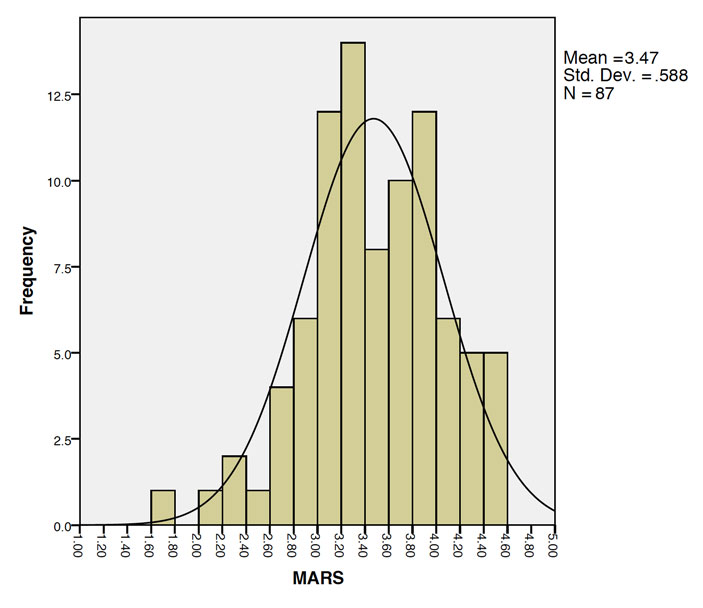
\includegraphics[scale=0.4, angle=0]{Files/prevention-study-2/figures/allapps-histogram}
    \caption{Histogram showing distribution and normal curve of mean MARS scores for all 87 reviewed apps.}
    \label{fig: allapps-histogram}
\end{figure}

\begin{figure}[h]
    \centering
    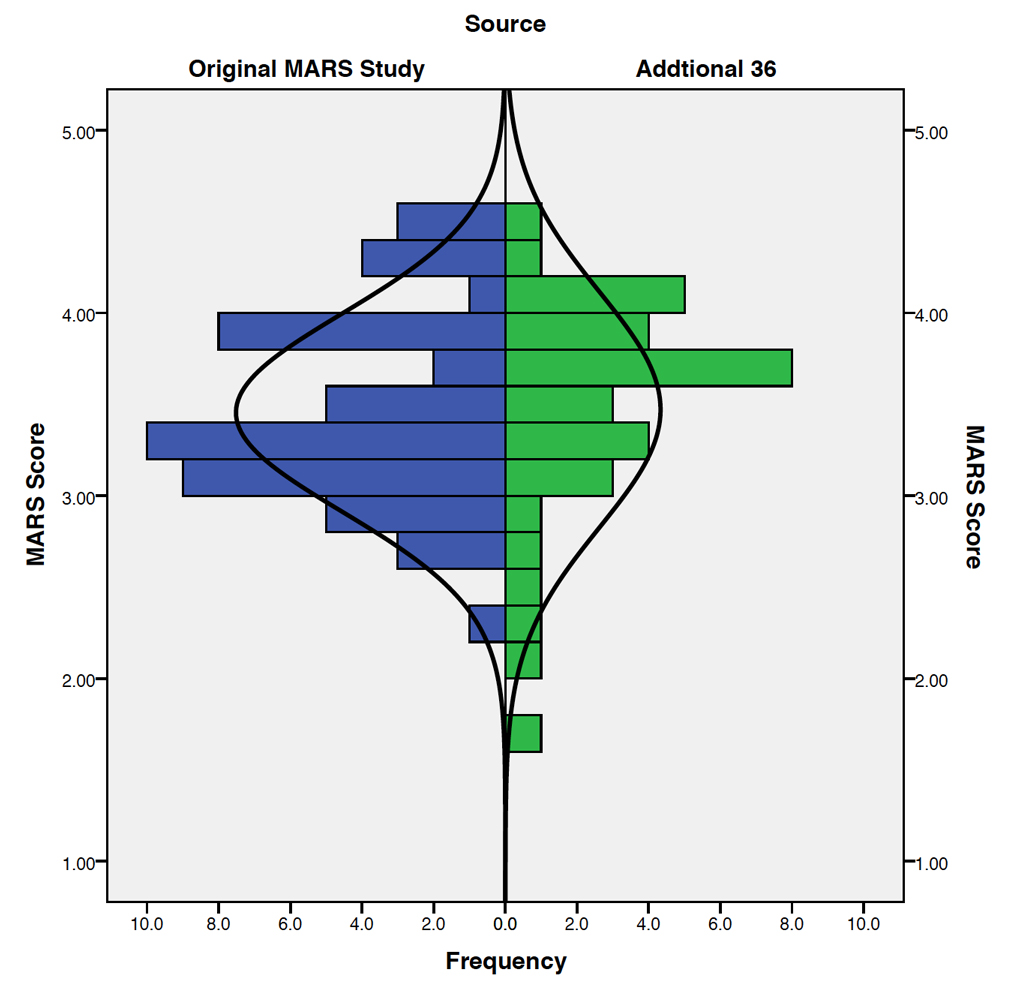
\includegraphics[scale=0.30, angle=0]{Files/prevention-study-2/figures/allapps-histogram-bysource}
    \caption{Histogram showing distribution and normal curve of mean MARS scores for all 87 reviewed apps segregated by source.}
    \label{fig: allapps-histogram}
\end{figure}

Whilst the apps can be ranked against one another using the MARS score, the reasons for the score are still not fully understood. To understand the factors which influence the rankings content analysis is performed on all 87 apps.

\section{Content Analysis} \label{subsection: content-analysis}
All 87 apps were downloaded, used, and studied by the author to glean information as to the various approaches used. This included establishing the primary behavioural domain targeted, if multiple domains were addressed, the format of educational information, the method of behavioural tracking (if applicable), if behavioural goals were recommended and if progression was structured/guided.

Correlation and regression analysis was performed on all observed content. Correlation analysis was used to determine if there was a relation between two or more variables, and to what degree. Regression analysis was used to establish if one variable (i.e. Number of domains addressed) could predict the outcome of another (i.e. MARS score). In addition, analysis of variance (ANOVA) was used to determine if there was a significant difference in results between two or more independent groups (e.g. Educational format used and Mean Education score).
%VIVA: Why not multiple variables in the regression model?

\subsection{Domains Targeted}
%Pairs of domains targeted commonly found together?
Apps were analysed to establish which behavioural domains they targeted. In cases where an app targeted more than 1 domain, a primary domain was established. Descriptives of this analysis can be found in Table \ref{tbl: descriptive-primarydomain-mars}. A count of targeted domains was also calculated.

\begin{table}[h]
\centering
\caption{Descriptive statistics of MARS score by primary domain targeted.}
\label{tbl: descriptive-primarydomain-mars}
\begin{tabular}{@{}lllllllll@{}}
\toprule
 &  &  &  &  & \multicolumn{2}{l}{95\% CI for Mean} &  &  \\ \cmidrule(lr){6-7}
\begin{tabular}[c]{@{}l@{}}Primary\\ Domain\end{tabular} & N & Mean & \begin{tabular}[c]{@{}l@{}}Std. \\ Dev.\end{tabular} & \begin{tabular}[c]{@{}l@{}}Std. \\ Error\end{tabular} & \begin{tabular}[c]{@{}l@{}}Lower\\ Bound\end{tabular} & \begin{tabular}[c]{@{}l@{}}Upper\\ Bound\end{tabular} & Min. & Max. \\ \midrule
Physical & 12 & 3.7017 & .46501 & .13424 & 3.4062 & 3.9971 & 3.01 & 4.45 \\
Diet & 9 & 3.7322 & .51558 & .17186 & 3.3359 & 4.1285 & 3.09 & 4.49 \\
Cognitive & 9 & 3.3967 & .96903 & .32301 & 2.6518 & 4.1415 & 1.67 & 4.51 \\
Sleep & 7 & 3.1514 & .29311 & .11079 & 2.8803 & 3.4225 & 2.73 & 3.53 \\
Stress & 41 & 3.4561 & .51771 & .08085 & 3.2927 & 3.6195 & 2.22 & 4.49 \\
Social & 5 & 2.9420 & .79408 & .35513 & 1.9560 & 3.9280 & 2.00 & 3.90 \\
Smoking & 4 & 3.7775 & .29590 & .14795 & 3.3067 & 4.2483 & 3.43 & 4.11 \\ \midrule
Total & 87 & 3.4731 & .58904 & .06315 & 3.3476 & 3.5986 & 1.67 & 4.51 \\ \bottomrule
\end{tabular}
\end{table}

One-way ANOVA was used to compare the effect of the primary domain targeted on the MARS score. ANOVA analysis showed there was no significant effect of the primary domain on the MARS Score at the p\textless.05 level [F(6, 80) = 1.946, p = 0.083].
Correlation analysis showed that the number of domains targeted and MARS score were significantly positively correlated at the p\textless.05 level (r = .257, p = .017). Linear regression analysis indicated that the number of domains targeted explained a significant amount of the variance in the MARS scores [F(1, 84) = 5.933, p = .017, R\textsuperscript{2} = .066, R\textsuperscript{2}\textsubscript{Adjusted} = .055]. For every additional domain, the MARS score increased by 0.153. The resultant linear regression equation is as follows:

\begin{equation}
MARSscore = 3.261 + 0.153 \left(NumDomains\right)
          \label{eq: calc-performance-stars}
\end{equation}

\subsection{App Service Types}
Apps were categorised into 5 main types, based on the service they provided: (1) Tracking, (2) Education, (3) Delivery, (4) Gaming, and (6) Multi.

\textit{Tracking} apps provided the facility to longitudinally track actions, behaviours or body-measurements, for the purpose of analysis, either by self or software.
\newline \textit{Education} apps provided strictly educational information on a specific topic.
\newline \textit{Delivery} apps aimed to deliver a service, experience, or content that was not strictly educational, nonetheless, was typically entertaining.
\newline \textit{Gaming} apps delivered interactive games, typically math or language puzzles.
\newline \textit{Multi} apps encompassed 2 or more app types, e.g. Tracking, Education and Gaming. These apps were typically more complex, and developed by established software development houses.

\begin{table}[h]
\centering
\caption{Descriptive Statistics of MARS score by Service Type.}
\label{tbl: descriptive-servicetype-mars}
\begin{tabular}{@{}lllllllll@{}}
\toprule
 &  &  &  &  & \multicolumn{2}{c}{95\% CI for Mean} &  &  \\ \cmidrule(lr){6-7}
\begin{tabular}[c]{@{}l@{}}Service \\ Type\end{tabular} & N & Mean & \begin{tabular}[c]{@{}l@{}}Std. \\ Dev.\end{tabular} & \begin{tabular}[c]{@{}l@{}}Std. \\ Error\end{tabular} & \begin{tabular}[c]{@{}l@{}}Lower\\ Bound\end{tabular} & \begin{tabular}[c]{@{}l@{}}Upper \\ Bound\end{tabular} & Min. & Max. \\ \midrule
Multi & 8 & 4.0638 & .31785 & .11238 & 3.7980 & 4.3295 & 3.71 & 4.51 \\
Delivery & 38 & 3.3339 & .48253 & .07828 & 3.1753 & 3.4926 & 2.22 & 4.49 \\
Tracking & 28 & 3.6050 & .45689 & .08634 & 3.4278 & 3.7822 & 2.67 & 4.45 \\
Education & 8 & 3.3225 & .87891 & .31074 & 2.5877 & 4.0573 & 2.00 & 4.41 \\
Game & 5 & 3.0880 & 1.06500 & .47628 & 1.7656 & 4.4104 & 1.67 & 4.29 \\ \midrule
Total & 87 & 3.4731 & .58904 & .06315 & 3.3476 & 3.5986 & 1.67 & 4.51 \\ \bottomrule
\end{tabular}
\end{table}

The developed Gray Matters app was classified as a \textit{Multi} app, due to its service delivery in Education, Tracking and Delivery. As shown in Table \ref{tbl: descriptive-servicetype-mars}, the majority of apps were classified as delivery and tracking apps, and less than 10\% were considered Multi apps.
In this case, one-way ANOVA was used to compare the effect of the service type on the MARS score. ANOVA analysis showed that there was a significant effect of service type on the MARS Score at the p\textless.05 level [F(4, 82) = 4.064, p = 0.05]. Post hoc comparisons using the Bonferroni test indicated that the mean score for Multi type apps (M = 4.06, SD = 0.31) was significantly different than Delivery (M = 3.33, SD = 0.48, p=0.011) and Game (M = 3.08, SD = 1.06, p=0.028). This is presented in Figure \ref{fig: servicetype-mars-anova}. No significance was found between Tracking or Education with any other service type.

\begin{figure}[h]
    \centering
    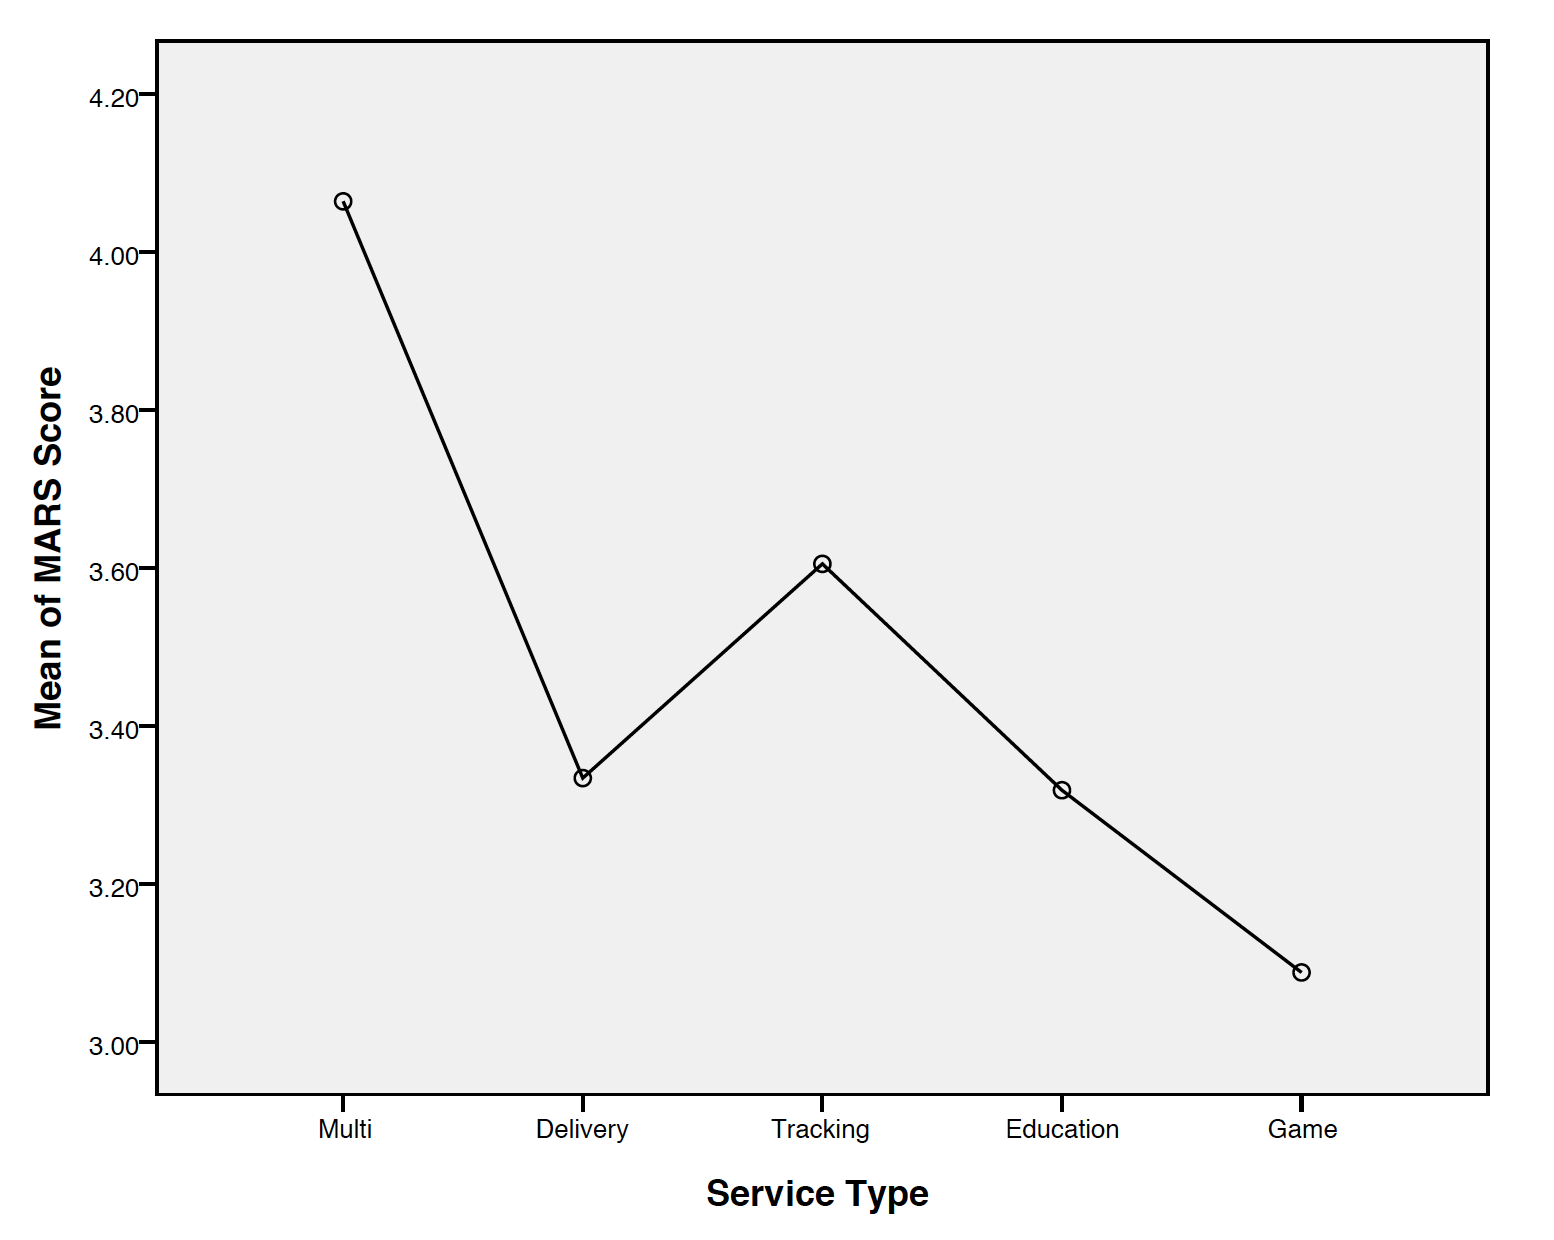
\includegraphics[scale=0.40, angle=0]{Files/prevention-study-1/figures/servicetype-mars-anova}
    \caption{Mean plot showing MARS score for apps based upon service type.}
    \label{fig: servicetype-mars-anova}
\end{figure}

\subsection{Education Format}
Apps were analysed to determine if they contained educational information, and if so, in which formats (i.e. text, image, audio, video, graphs, and human coaching).
Comparing apps which had an education component, with those that had not, using an independent samples t-test showed no significant difference in overall MARS score. There was however, a significant difference found in the information sub-scores for educational (M = 3.23, SD = .904 ) and non-educational apps (M = 2.82, SD = .916) at the p\textless.05 level [t(85) = -2.00, p = 0.048].
Further analysis of apps which contain educational information (n=56), showed that over 75\% used text as a method to provide educational information. Further details of formats and their frequencies can be found in Table \ref{tbl: educationformat-frequencies}.
%VIVA: Chris comment - I am just thinking – if asked,  how will you be able to defend your choice of MARS as a validated tool and also as a choice of other methods which may have been available?

\begin{table}[h]
\centering
\caption{Frequencies of information format within apps that provided educational material.}
\label{tbl: educationformat-frequencies}
\begin{tabular}{@{}lll@{}}
\toprule
Education Format & Frequency & \% \\ \midrule
Text & 44 & 78.6 \\
Image & 13 & 23.2 \\
Audio & 18 & 32.1 \\
Video & 11 & 19.6 \\
Graph & 2 & 3.6 \\
Coach & 3 & 5.6 \\ \bottomrule
\end{tabular}
\end{table}

An independent samples t-Test was conducted to compare MARS scores (including criteria sub-scores) in apps using text and no text. There was a significant difference in the MARS scores for apps using text (M = 3.63, SD = .579) or no text (M = 3.30, SD = .556) as an educational format [t(85) = -2.73, p = 0.08]. A similar result was found in apps using images and no images. There was a significant difference in the MARS scores for apps using images (M = 3.95, SD = .315) or no images (M = 3.38, SD = .585) as an educational format [t(85) = -3.58, p = 0.001]. No significant difference in MARS score was found in apps using or not using audio, video, graphs or human coaches.

These results suggest that textual information has an effect on the overall MARS rating. Specifically, the results suggest that using text to deliver educational information has a positive effect on the perceived efficacy of the app for the purposes of improving health.

\subsection{Tracking Methods}
Apps were analysed to establish if they facilitated tracking health metrics or behaviours, and if so, how this was performed. Forms of tracking were categorised as:
\begin{enumerate}[noitemsep,topsep=0pt]
\item \textbf{manual} self-tracking.
\item \textbf{automatic} tracking via smartphone sensors (e.g. step counter app).
\item structured program \textbf{progression}.
\item tracking via \textbf{connected} devices (e.g. wrist-worn activity monitors).
\end{enumerate}

52.0\% (n=46) of the apps reviewed facilitated some form of behavioural or health tracking. Frequencies of the tracking methods used within these apps have been presented in Table \ref{tbl: trackingtype-frequencies}. The majority of apps facilitate manual self-reporting. A potential reason for this is that whilst onboard sensors and connected wearables may detect and quantify physical activity and vital signs, self-reporting is the only method from which to extract qualitative measures, including perceptions of mood and stress.

\begin{table}[h]
\centering
\caption{Frequencies of tracking methods within apps that provided educational material.}
\label{tbl: trackingtype-frequencies}
\begin{tabular}{@{}lll@{}}
\toprule
Tracking Method & Frequency & \% \\ \midrule
Manual & 34 & 73.9 \\
Automatic & 3 & 6.5 \\
Progression & 4 & 8.7 \\
Connected & 4 & 8.7 \\ \bottomrule
\end{tabular}
\end{table}

The majority of the apps that facilitate tracking do so using only one method (89.1\%, n=41). An independent samples t-Test was conducted to compare MARS scores (including criteria sub-scores) in apps that facilitated tracking and those that did not. There was a significant difference in the MARS scores for apps that facilitated tracking (M = 3.73, SD = .464) and apps that did not (M = 3.17, SD = .579) [t(85) = -4.96, p = \textless0.00].
Statistical significance was also found within tracking/no tracking comparisons for the Engagement, Aesthetics and Subjective sub-criteria.
\newline There was a significant difference in the \textit{engagement} scores for apps that facilitated tracking (M = 3.57, SD = .711) and apps that did not (M = 2.54, SD = .768) [t(85) = -6.48, p = \textless0.00]. Significance in \textit{aesthetics} scores for apps that facilitated tracking (M = 4.07, SD = .755) and apps that did not (M = 3.30, SD = .726) [t(85) = -4.89, p = \textless0.00] and \textit{subjective} scores for apps that facilitated tracking (M = 3.28, SD = .954) and apps that did not (M = 2.01, SD = .626) [t(78.4) = -7.42, p = \textless0.00]. No significant difference was found in the functionality and information criteria scores.
A number of apps utilised more than one tracking method, as such, the quantity of tracking methods utilised by each app and tested for correlation with MARS scores. In apps that facilitated tracking (n=45), the quantity of tracking methods utilised showed no correlation with the MARS score (r = .056, p = .716).
These results suggest that facilitating the tracking of behaviours has a significant effect on the overall MARS rating score, which is directly affected by the engagement and aesthetic criteria scores. Upon the inclusion of a single tracking method, the quantity of tracking methods does not influence score, regardless of type.

\subsection{Structured Progression}
Apps were examined to establish if they provided a structured progression program, helping to guide users through various states or stages of the apps activity. For example, increasing physical activity goal values once previous goals are met, controlling exposure to difficult goals, or simply providing increasingly detailed information on a specific topic as the user becomes better informed. Of the apps reviewed, 32.2\% (n=28) were categorised as enabling structured progression.
An independent samples t-Test was conducted to compare MARS scores (including criteria sub-scores) in apps that were structured and not structured. There was a significant difference in the MARS scores for apps that were structured (M = 3.80, SD = .458) and not structured (M = 3.31, SD = .581) [t(85) = -3.90, p = \textless0.00]. Statistical significance between structured and not structured apps was also found within the Engagement, Aesthetics, Information and Subjective sub-criteria scores.
\newline Significance in \textit{engagement} scores that were structured (M = 3.58, SD = .925) and not structured (M = 2.84, SD = .784) [t(85) = -3.87, p = \textless0.00].
\newline Significance in \textit{aesthetics} scores that were structured (M = 4.16, SD = .728) and not structured (M = 3.49, SD = .797) [t(85) = -3.75, p = \textless0.00].
\newline Significance in \textit{information} scores that were structured (M = 3.39, SD = .615) and not structured (M = 2.94, SD = 1.01) [t(79.67) = -2.60, p = \textless0.00].
\newline Significance in \textit{subjective} scores that were structured (M = 3.28, SD = 1.15) and not structured (M = 2.39, SD = .837) [t(40.8) = -3.6, p = 0.01]. No significant difference was found in the functionality criteria.

These results suggest that including a form of structured progression within the app has a significantly positive effect on the overall MARS rating, including ratings of engagement, aesthetics, and information.

\subsection{Gamification Methods}
Apps were examined to establish if they contained elements of gamification, which included points, goals, achievements, rankings, and social competition. 34.5\% (n=30) of apps analysed implemented elements of gamification, with over 50\% (n=16) of these apps using more than 1 gamification element.
The most common gamification elements used were points, achievements and targets as presented in Table \ref{tbl: gamification-frequency}.

\begin{table}[h]
\centering
\caption{Frequencies of gamification elements within apps that implemented gamification.}
\label{tbl: gamification-frequency}
\begin{tabular}{@{}lll@{}}
\toprule
Element & Frequency & \% \\ \midrule
Points               & 17        & 56.7     \\
Targets              & 16        & 53.3     \\
Achievements         & 15        & 50      \\
Rankings             & 6         & 20       \\
Social               & 4         & 13.3         \\ \bottomrule
\end{tabular}
\end{table}

Apps were analysed to establish if they provided a structured progression program, helping to guide users through various states or stages of the apps activity. An independent samples t-Test was conducted to compare MARS scores (including criteria sub-scores) in apps that had elements of gamification and no gamification. There was a significant difference in the MARS scores for gamification apps (M = 3.85, SD = .468) and no gamification app (M = 3.27, SD = .545) [t(85) = -5.018, p = \textless0.00]. Statistical significance between apps who implemented gamification, and those that did not, was also found within the Engagement, Aesthetics, and Subjective sub-criteria scores.
Significance in \textit{engagement} scores for gamification apps (M = 3.79, SD = .626) and no gamification app (M = 2.71, SD = .788) [t(85) = -6.50, p = \textless0.00]. Significance in \textit{aesthetics} scores for gamification apps (M = 4.29, SD = .628) and no gamification app (M = 3.40, SD = .765) [t(85) = -5.45, p = \textless0.00]. Significance in \textit{subjective} for gamification apps (M = 3.57, SD = .895) and no gamification app (M = 2.21, SD = .756) [t(85) = -7.47, p = \textless0.00]. No significant difference was found in the functionality or information criteria.

These results suggest that including gamification within the app has a significantly positive effect on the overall MARS rating, including ratings of engagement, aesthetics, and subjectivity.

The gamification elements were then examined to determine if the use of certain elements had an effect on the MARS score. An independent samples t-Test of apps that used at least one gamification element (n=30) showed a significant difference in MARS scores for apps that used achievements (M = 4.06, SD = .316), and those that did not (M = 3.65, SD = .511) [t(28) = -2.68, p = 0.12]. Although not statistically significant, there was a notable difference in engagement scores between apps that used points (M = 3.97, SD = .628), and those that did not (M = 3.56, SD = .569) [t(28) = -1.8, p = 0.08]. The remaining gamification types displayed no significant differences within independent samples t-Tests.

%Examine if gamification method determines score?
%Game methods vs each other
%Gamification vs rest

Correlation analysis showed that the number of gamification elements used and MARS score were significantly positively correlated at the p\textless.05 level (r = .518, p = \textless0.00). Linear regression analysis shows that the number of domains targeted explain a significant amount of the variance in the MARS scores [F(1, 85) = 22.5, p = \textless0.00, R\textsuperscript{2} = .210, R\textsuperscript{2}\textsubscript{Adjusted} = .200]. For every additional gamification element used, the MARS score increased on average by 0.235. The linear regression line is presented in Figure \ref{fig: gamification-regression} and the equation is as follows:

\begin{equation}
MARSscore = 3.316 + 0.235 \left(NumberGamificationElements\right)
          \label{eq: calc-performance-stars}
\end{equation}

\begin{figure}[h]
    \centering
    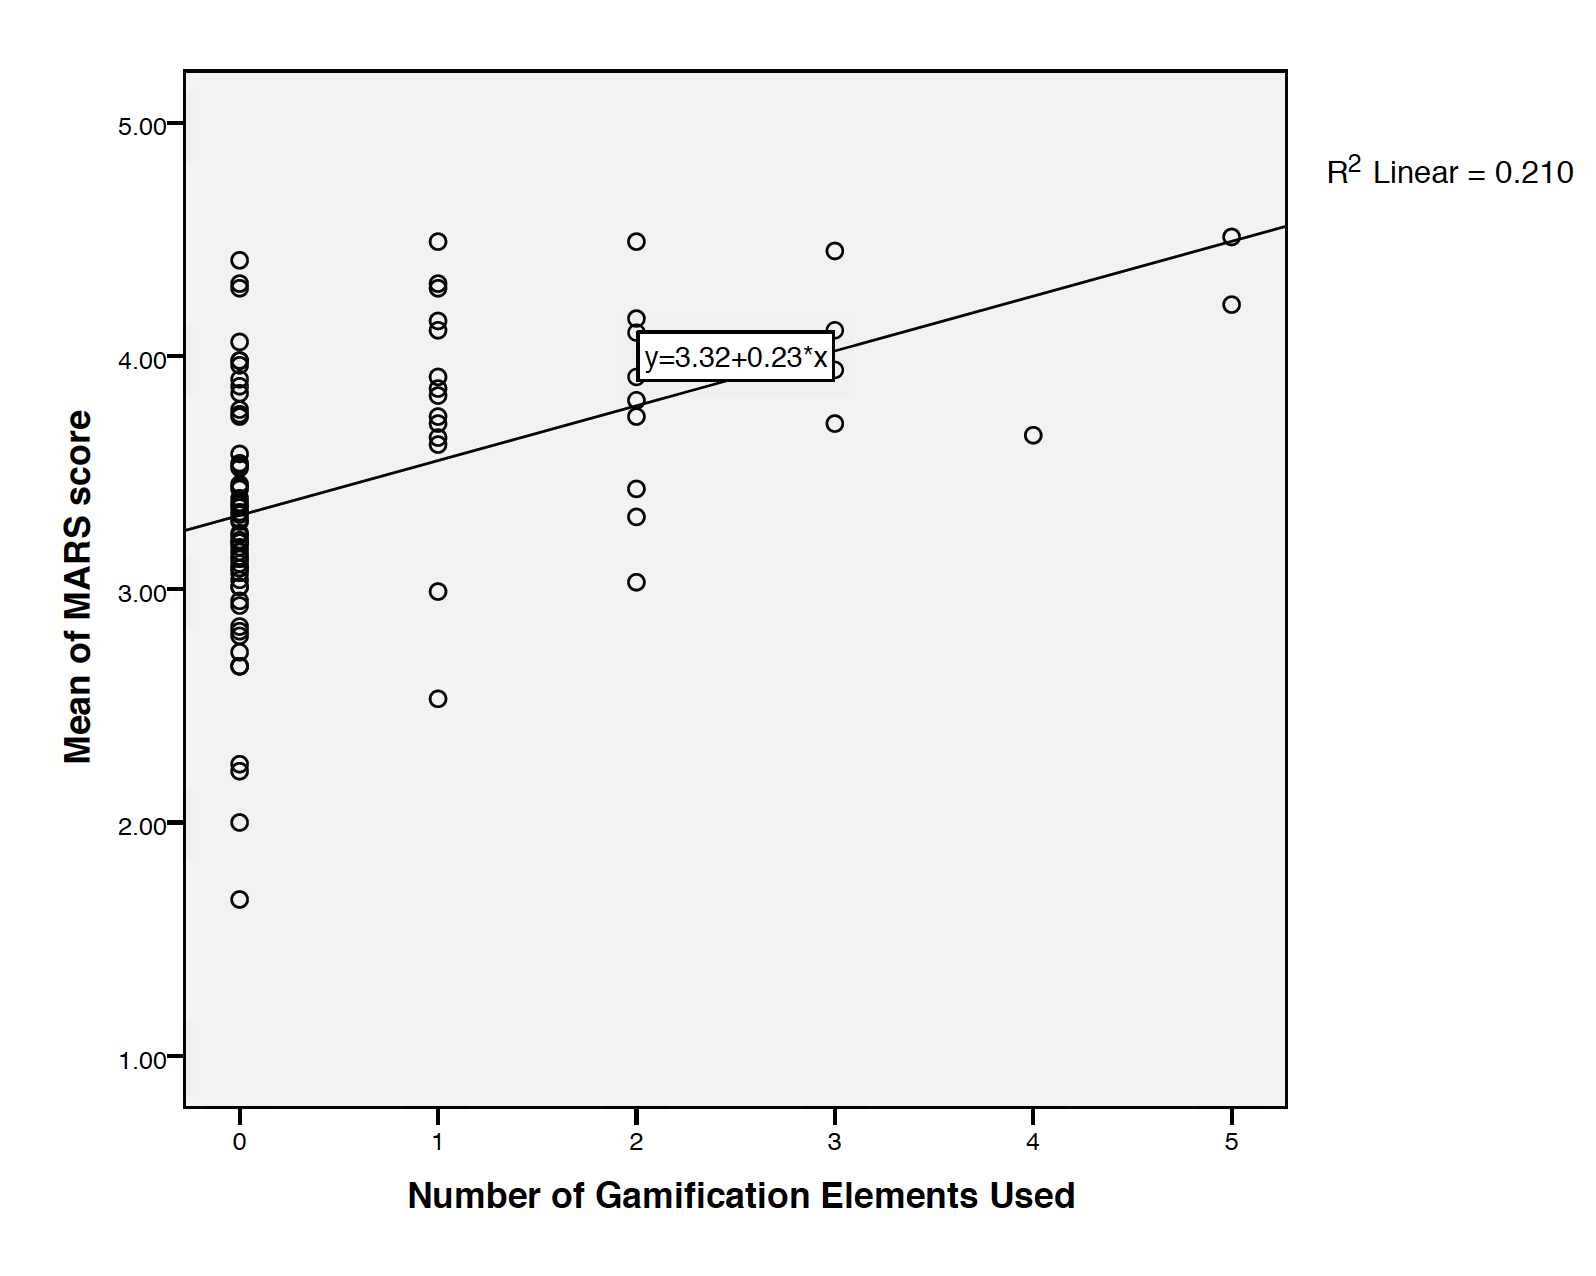
\includegraphics[scale=0.40, angle=0]{Files/prevention-study-1/figures/gamification-regression}
    \caption{Scatter plot showing MARS score against Number of Gamification elements used.}
    \label{fig: gamification-regression}
\end{figure}

\subsection{Social Integration} \label{subsection: social-integration}
Each app was analysed to determine if it integrated any form of social media or networking. Examples of social integration include the creation of a friend network, sharing gamification points with friends, sharing progression with existing social networking contacts, comparison of results with friends. Of the apps reviewed, 23\% (n=20) implemented social elements, the remaining 73\% (n=67) did not. An independent samples t-Test was conducted to compare MARS scores (including criteria sub-scores) in apps that integrated social elements and those that did not. There was a significant difference in the MARS scores for social apps (M = 3.83, SD = .457) and not social (M = 3.36, SD = .584) [t(85) = -3.73, p = 0.002]. Statistical significance was also found within the Engagement, Aesthetics, and Subjective criteria scores.
Significance at the p \textless 0.05 level was found between \textit{engagement} scores for social apps (M = 3.83, SD = .713) and non-social apps (M = 2.86, SD = .828) [t(85) = -4.70, p = \textless0.00]. Significance at the p \textless 0.05 level was found between \textit{aesthetics} scores for social apps (M = 4.21, SD = .686) and non-social apps (M = 3.56, SD = .818) [t(85) = -3.246, p = 0.002]. Significance at the p \textless 0.05 level was found between \textit{subjective} for social apps (M = 3.50, SD = .833) and non-social apps (M = 2.43, SD = .961) [t(85) = -4.49, p = \textless0.00]. No significant difference was found in the functionality or information criteria.

Results suggest that integrating social elements within an app will positively affect the overall MARS score, including engagement, aesthetics, and subjective criteria scores.

\subsection{Media Use and Format}
In a similar fashion to how the analysis of education format was performed, each app was also analysed for the use of various forms of media, including audio, video, image, graphs, and games. 78\% (n=68) of the apps used some form of media to represent or deliver content to the user. The frequencies of each format can be found in Table \ref{tbl: mediaformat-frequencies}. Excluding apps with no media, 72.1\% (n=49) of the media apps used only one format, 17.6\% (n=12) used 2, and 10.3\% (n=7) used 3 or more.  Correlation analysis showed that the number of formats used and the MARS score were significantly positively correlated at the p\textless.05 level (r = .309, p = 0.01).

\begin{table}[h]
\centering
\caption{Frequencies of media types used format within apps that used media.}
\label{tbl: mediaformat-frequencies}
\begin{tabular}{@{}lll@{}}
\toprule
Media Format & Frequency & \% \\ \midrule
Image & 32 & 47.1 \\
Audio & 31 & 45.6 \\
Video & 13 & 19.1 \\
Graph & 14 & 20.6 \\
Games & 8 & 11.8 \\ \bottomrule
\end{tabular}
\end{table}

Using an independent samples t-Test no significance was found in the MARS score, or criteria sub-scores, between the use of media and not. There was, however, significance found in various sub-scores and the use of certain media formats. There was a significant difference found in subjective scores in the use of audio (M = 2.86, SD = 1.02), and not (M = 2.35, SD = .970) [t(85) = 2.253, p = 0.027].
There was a significant difference found through the use of images and not, in the \textit{aesthetics} score (No Image = 3.50, SD = .815,  Image: M = 4.06, SD = .754) [t(85) = -3.14, p = 0.002], the \textit{engagement} score (No image: M = 2.93, SD = .835, Image: M = 3.36, SD = .945) [t(85) = -2.23, p = 0.028], and overall \textit{MARS} score (No image: M = 3.37, SD = .630, Image: M = 3.64, SD = .470) [t(85) = -2.14, p = 0.035].
There was also a significant difference found in the use of graphs, and not, in the \textit{aesthetics} score (No graph: M = 3.62, SD = .832, Graph: M = 4.17, SD = .470) [t(85) = -2.34, p = 0.021], and in the \textit{subjective} score (No graph: M = 2.51, SD = .986, Graph: M = 3.57, SD = .805) [t(85) = -3.77, p = \textless0.00].
In addition, a significant difference in \textit{engagement} scores were found in apps who used games (M =  3.02, SD = .86), and those that did not (M = 3.75, SD = 1.04) [t(85) = -2.24, p = 0.28].

These results indicate that the addition of specific visual formats, i.e. Images, Graphs and Games can increase sub-criteria scores. Conversely, the inclusion of auditory formats can decrease ratings in the subjective criteria. Note, however, that the subjective is not taken into consideration when calculating the MARS score, so the importance is somewhat debatable.

\subsection{Condition Focus}
Of the 87 apps, 12 (13.8\%) apps focus on a specific health condition, with the remaining 75 (86.2\%) stating to improve health in a general sense. Of the condition focused apps (n=12), conditions targeted are AD (n=4, 33\%), Depression (n=2, 16.7\%), Insomnia (n=2, 16.7\%), Post Traumatic Stress Disorder (PTSD) (n=1, 8.3\%), Anorexia (n=1, 8.3\%), Suicide Prevention (n=1, 8.3\%), and Controlling Blood Pressure (n=1, 8.3\%). An independent samples t-Test was conducted to compare MARS scores (including criteria sub-scores) in apps that focused on a health condition and those that did not. There was no significant difference found between the groups at the p \textless 0.05 level.
One-way ANOVA was used to compare the effect of the condition focus type on the MARS score. ANOVA analysis showed there was no significant difference between the groups. Further analysis was then performed, removing groups which had fewer than 2 cases. The remaining apps were specifically focused on AD (n = 4, M = 3.36), Depression (n = 2, M = 2.95), and Insomnia (n = 2, M = 2.93). No significant difference was found between the groups in the MARS scores or any criteria sub-scores.

\subsection{Pricing}
Each app's price was categorised based upon its cost to the user. Apps were categorised as Free (61.8\%), Paid (8.8\%), Subscription (4.4\%), and In-App (25\%). Free apps do not incur any cost to download or use. Paid apps are those that incur a one-time fee to download the app, after which it belongs to the user. Subscription apps are free to download, however, are based upon a service delivery model, whereby the user pays to use the app on a time or service based quota. The In-App category describes apps that are free to download, however, have additional content that can be purchased to supplement or expand upon the originally free material.
One-way ANOVA was used to compare the effect of the pricing type on the MARS score. ANOVA analysis showed there was a significant effect of pricing type on the MARS Score at the p\textless.05 level [F(3, 83) = 4.521, p = 0.05]. Post hoc comparisons using the Bonferroni test indicated that the mean score for Subscription type apps (M = 4.20, SD = 0.214) was significantly different than Free (M = 3.39, SD = 0.60, p=0.016) and Paid apps (M = 3.14, SD = 0.478, p=0.010). This is presented in Figure \ref{fig: pricetype-mars-anova}. An independent samples t-Test between apps that use the subscription pricing model, and those that do not, highlighted that a significantly larger proportion of subscription apps implemented structured progression (M = .80, SD = .447), than other pricing types (M = .29, SD = .458) [t(85) = -2.40, p = 0.18]. As with previous analysis, the inclusion of structured progression is associated with increased MARS scores.

Further analysis was performed between apps that used the subscription model (n=5), and those that did not (n=82). A Pearson's Chi-Square test was performed which showed that the subscription model was significantly related to the use of structured progression (x\textsuperscript{2}(1) = 5.557, p = 0.018, Cramer's V = .253). Only 29.3\% of other pricing types implemented structured progression, whilst 80\% of subscription apps implemented structured progression, which had been previously shown to positively affect the MARS score.

\begin{figure}[h]
    \centering
    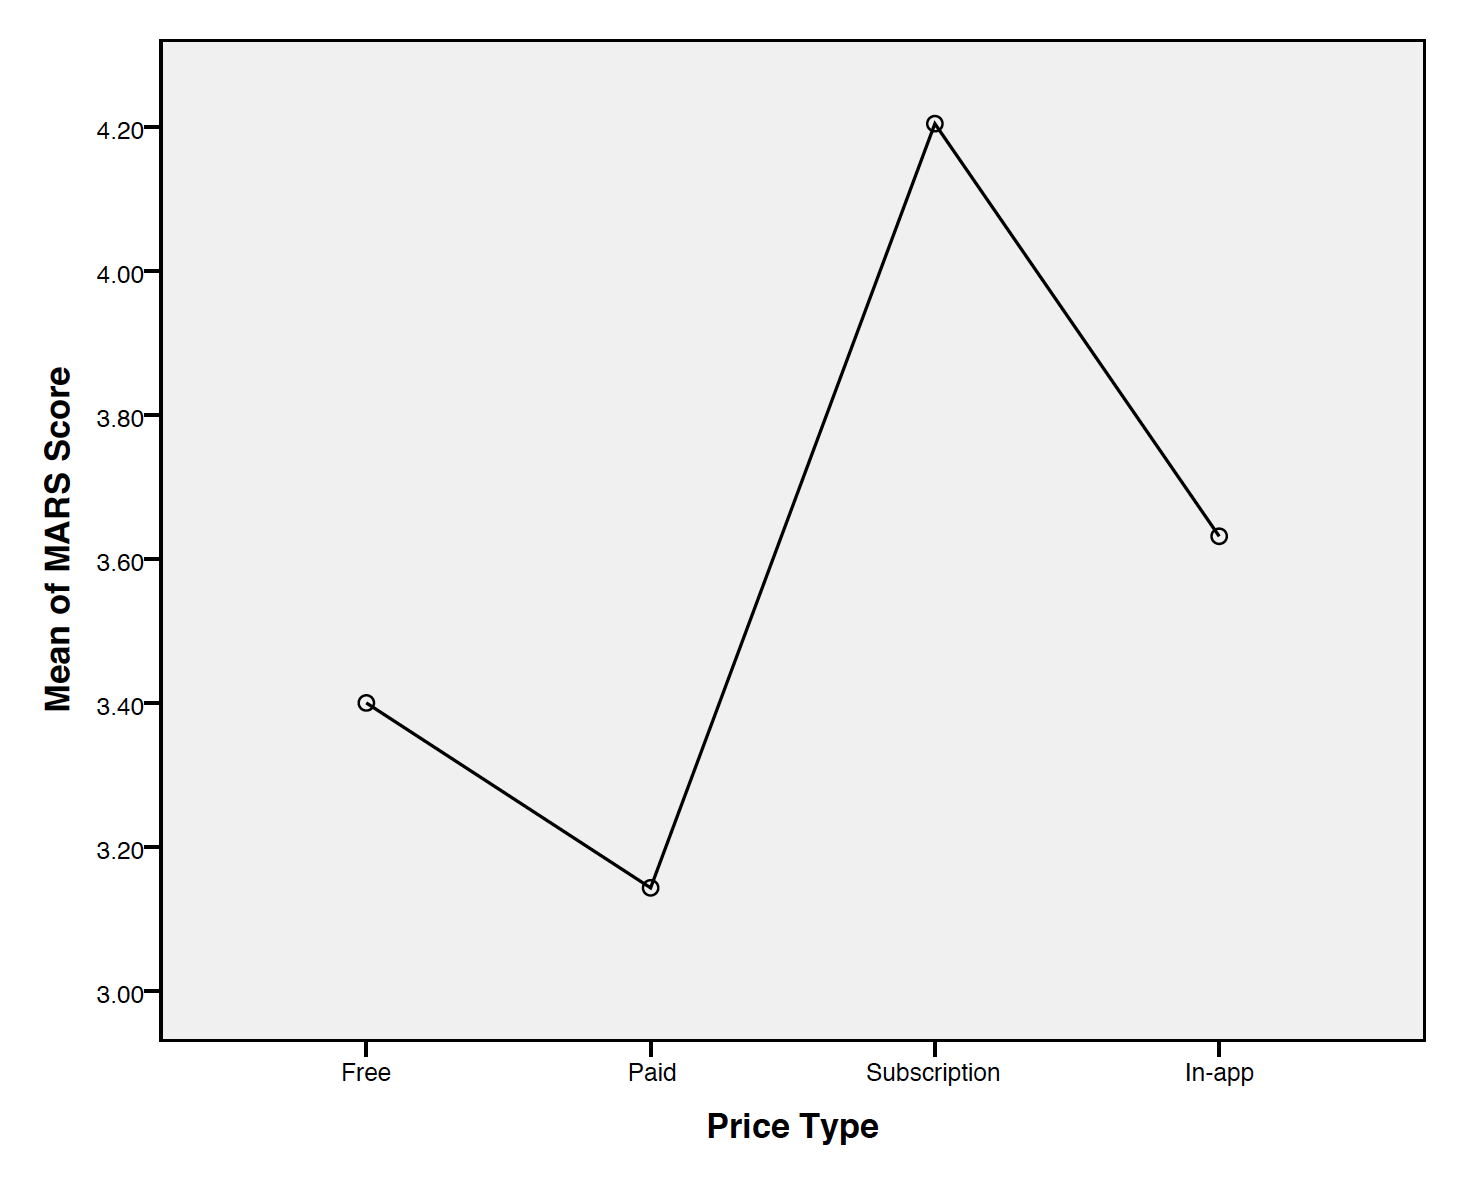
\includegraphics[scale=0.40, angle=0]{Files/prevention-study-1/figures/pricetype-mars-anova}
    \caption{Mean plot showing the MARS score for Price types.}
    \label{fig: pricetype-mars-anova}
\end{figure}

\subsection{Discussion} \label{subsection: MARS-discussion}
From analysing the elements within each app, a number of important observations were made. The inclusion of certain elements had a significantly positive effect on the overall MARS score, often influenced by significant impact in criteria sub-scores. The following summarises the observations:

\begin{enumerate}[noitemsep,topsep=0pt]
\item Targeting \textbf{multiple domains} results in a significantly higher MARS score.
\item Providing \textbf{more than one primary service} results in a significantly higher MARS score.
\item Providing \textbf{educational information} significantly increases information scores.
\item Inclusion of \textbf{text as an education format} significantly increases MARS score in all apps.
\item The \textbf{use of images} to supplement education material significantly increases MARS scores.
\item \textbf{Facilitating tracking} significantly increases engagement, aesthetics, subjective and overall MARS scores.
\item There is \textbf{no relation} between score and quantity of tracking methods.
\item Apps which provide a \textbf{structured program} have a significantly higher MARS, engagement, aesthetics, information, and subjective criteria scores.
\item Apps which \textbf{utilise elements of gamification} have significantly higher MARS, engagement, aesthetics, and subjective criteria scores.
\item Use of the \textbf{achievements} gamification element results in a significantly higher MARS score.
\item The \textbf{number of gamification elements} used was significantly positively correlated with the MARS score.
\item The integration of \textbf{social elements} result in a significantly higher MARS score.
\item No significant difference was found in apps that used \textbf{media and no media}.
\item In apps that used media, significant differences were found between the \textbf{media formats used}, with the highest scores resulting from the use of images, graphs and games.
\item The \textbf{number of media formats} used was significantly positively correlated with the MARS score.
\item No significant difference was found in any scoring metric within apps that \textbf{targeted a specific health condition}and those that did not.
\item Free apps were rated higher on average than one-off payment apps, however, lower than subscription and in-app purchase apps.
\item Apps which use a \textbf{subscription based pricing model} have a significantly higher MARS score.
\end{enumerate}

From these results it is clear that a number of recommendations may be made for an app which aims to score highly on the MARS scale. Such recommendations include the utilisation of multiple services addressing multiple behavioural domains, clear information delivery provided through numerous media formats, with a specific focus on imagery, facilitating tracking, and the inclusion of gamification elements, specifically the use of points and achievements.
%VIVA: Chris - Surely these will be subjective recommendations for MARS?
%VIVA: Phillip - Yes, the recommendations will be influenced by the MARS scoring, however, the scale was designed as a tool to rate mHealth apps. Expand further.

\subsubsection{The Gray Matters App}
The Gray Matters app incorporates many of the recommendations that have been uncovered through the content analysis in the previous section. The app targets 7 domains, provides educational material, facilitates tracking, facilitates structured progression, and implements gamification through point scoring. The app, however, does have a number of shortcomings; utilising only 1 form of education delivery (text), facilitating tracking through self-report only, and graphs are the only form of multimedia used.

\textbf{Regression Accuracy.} Using the regression equations from the number of domains targeted and number of gamification elements predicted that the MARS score would be 4.332, and 3.786 respectively.
Both scores underestimated the true score attributed by the expert reviewers of 4.53. This score however, is the result of only 5 expert reviewers, heavily skewed by the 4:1 Medicine:Computer Science ratio. Further research and recruitment of experts from neighbouring domains is needed to ensure the rating is valid.

\section{Conclusion}
This Chapter has presented the developed Gray Matters app's merit through expert review and contrast with existing apps, both in the commercial and research domain. Content analysis of 87 apps also uncovered valuable recommendations for the development of a successful mHealth app, and served to expose the current shortcomings of the Gray Matters app.
%VIVA: Chris - Why do you think the MARS study did not produce similar recommendations?
%VIVA: Phillip - The MARS study did not perform content analysis on the apps that they reviewed. I performed this work to further understand the factors which led to the ratings that were being agreed upon by the 'experts'.

